\newcommand{\lecturetitle}[1]{
  \title{01204211 Discrete Mathematics \\ #1}
  \author{Jittat Fakcharoenphol}
  \frame{\titlepage}
}

\lecturetitle{Lecture 15: Fibonacci sequence} 

\begin{frame}\frametitle{The Fibonacci sequence\footnote{This lecture mostly follows Chapter 4 of [LPV].}}

  \begin{columns}[c]
    \column{.3\textwidth}
    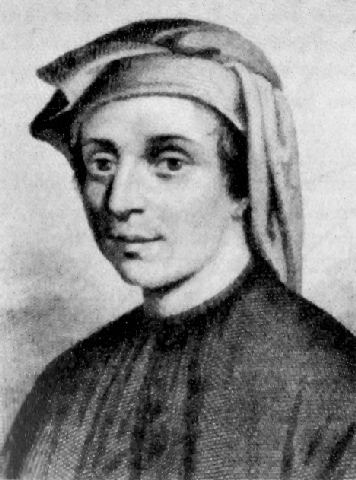
\includegraphics{images/fibonacci.jpg}

    {\tiny Source: https://en.wikipedia.org/wiki/ File:Fibonacci.jpg}
    
    \column{.7\textwidth}
    In 1202, Leonardo Bonacci (known as Fibonacci) asked the following
    question.

    \begin{tcolorbox}
      {\footnotesize ``[A]ssuming that: a newly born pair of rabbits,
        one male, one female, are put in a field; rabbits are able to
        mate at the age of one month so that at the end of its second
        month a female can produce another pair of rabbits; rabbits
        never die and a mating pair always produces one new pair (one
        male, one female) every month from the second month on.''

        ``The puzzle that Fibonacci posed was: how many pairs will
        there be in one year?''}
    \end{tcolorbox}
    
    {\tiny From https://en.wikipedia.org/wiki/Fibonacci\_number}
  \end{columns}
\end{frame}

\begin{frame}
  Let's try to solve Fibonacci's question. \pause

  Let $\spadesuit$ denote a newly born rabit pair, and $\heartsuit$
  denote a mature rabit pair.
  
  \begin{tabular}{c|l|r}
    Month & Rabits & \\ \hline
    1 & $\spadesuit$ & 1 \\ \pause
    2 & $\heartsuit$ & 1\\ \pause
    3 & $\heartsuit$ \pause $\spadesuit$ & 2 \\ \pause
    4 & $\heartsuit$ $\heartsuit$ \pause $\spadesuit$ & 3 \\ \pause
    5 & $\heartsuit$ $\heartsuit$ $\heartsuit$ \pause $\spadesuit$ $\spadesuit$ & 5 \\ \pause
    6 & $\heartsuit$ $\heartsuit$ $\heartsuit$ $\heartsuit$ $\heartsuit$ \pause $\spadesuit$ $\spadesuit$ $\spadesuit$ & 8 \\ \pause
    7 & $\heartsuit$ $\heartsuit$ $\heartsuit$ $\heartsuit$ $\heartsuit$ $\heartsuit$ $\heartsuit$ $\heartsuit$
    \pause $\spadesuit$ $\spadesuit$ $\spadesuit$  $\spadesuit$ $\spadesuit$ & 13
  \end{tabular}

  \vspace{0.1in}
  
  \pause How many rabit pairs do we have at the beginning of the 8th
  month? \pause

  {\small
    \begin{itemize}
    \item
      Surely all 13 rabit pairs we have in the 7th month remain there and
      are all mature.  So, the question is how many newly born rabbit
      pairs that we have. \pause
    \item
      The number of newly born rabbit pairs equals the number of mature
      rabbit pairs we have.  \pause This is also equal to the number of
      rabit pairs that we have in the 6th month: 8.
    \end{itemize}
  }
\end{frame}

\begin{frame}
  Thus, we will have 13+8 rabit pairs at the beginning of the 8th
  month.
  \pause
  
  If we write down the sequence, we get the Fibonacci sequence:
  \[
  1,1,2,3,5,8,13,21,\ldots
  \]
  \pause
  Again, what's the next number in this sequence?  How can you compute it? \pause

  21+13 = 34 is the answer. \pause You take the last two numbers and
  add them up to get the next number.  Why? 
\end{frame}

\begin{frame}
  To be precise, let $F_n$ be the $n$-th number in the Fibonacci
  sequence. (That is, $F_1=1, F_2=1, F_3=2, F_4=3$ and so on.)  We can
  define the $(n+1)$-th number as
  \[
  F_{n+1}=F_n+F_{n-1},
  \]
  for $n=2,3,\ldots$.
  \pause
  Is this enough to completely specify the sequence? \pause

  No, because we do not know how to start.  To get the Fibonacci
  sequence, we need to specify two starting values: $F_1=1$ and
  $F_2=1$ as well.

  Now, you can see that the equation and these special values uniquely
  determine the sequence.  It is also convenient to define $F_0=0$ so
  that the equation works for $n=1$.
\end{frame}

\begin{frame}\frametitle{A recurrence}
  The equation
  \[ F_{n+1}=F_n+F_{n-1} \]
  and the initial values $F_0=0$ and $F_1=1$ specify all values of the
  Fibonacci sequence.  With these two initial values, you can use the
  equation to find the value of any number in the sequence.

  This definition is called a {\bf recurrence}.  Instead of defining
  the value of each number in the sequence explicitly, we do so by
  using the values of other numbers in the sequence.
\end{frame}
